\documentclass[../Article_Sensitivity_Analsysis.tex]{subfiles}
\graphicspath{{\subfix{../Figures/}}}
\begin{document}
	
	\subsection{Flow rate}
	
	The increase in the mass-flow rate affects the system simultaneously along the spatial direction by increasing the velocity but without affecting the thermodynamic state of the fluid. As a result, Figure \ref{fig:Sensitivty_F_P} indicates that the system's pressure remains unaffected by changes in the flow rate.
	
	\begin{figure}[h!]
		\centering
		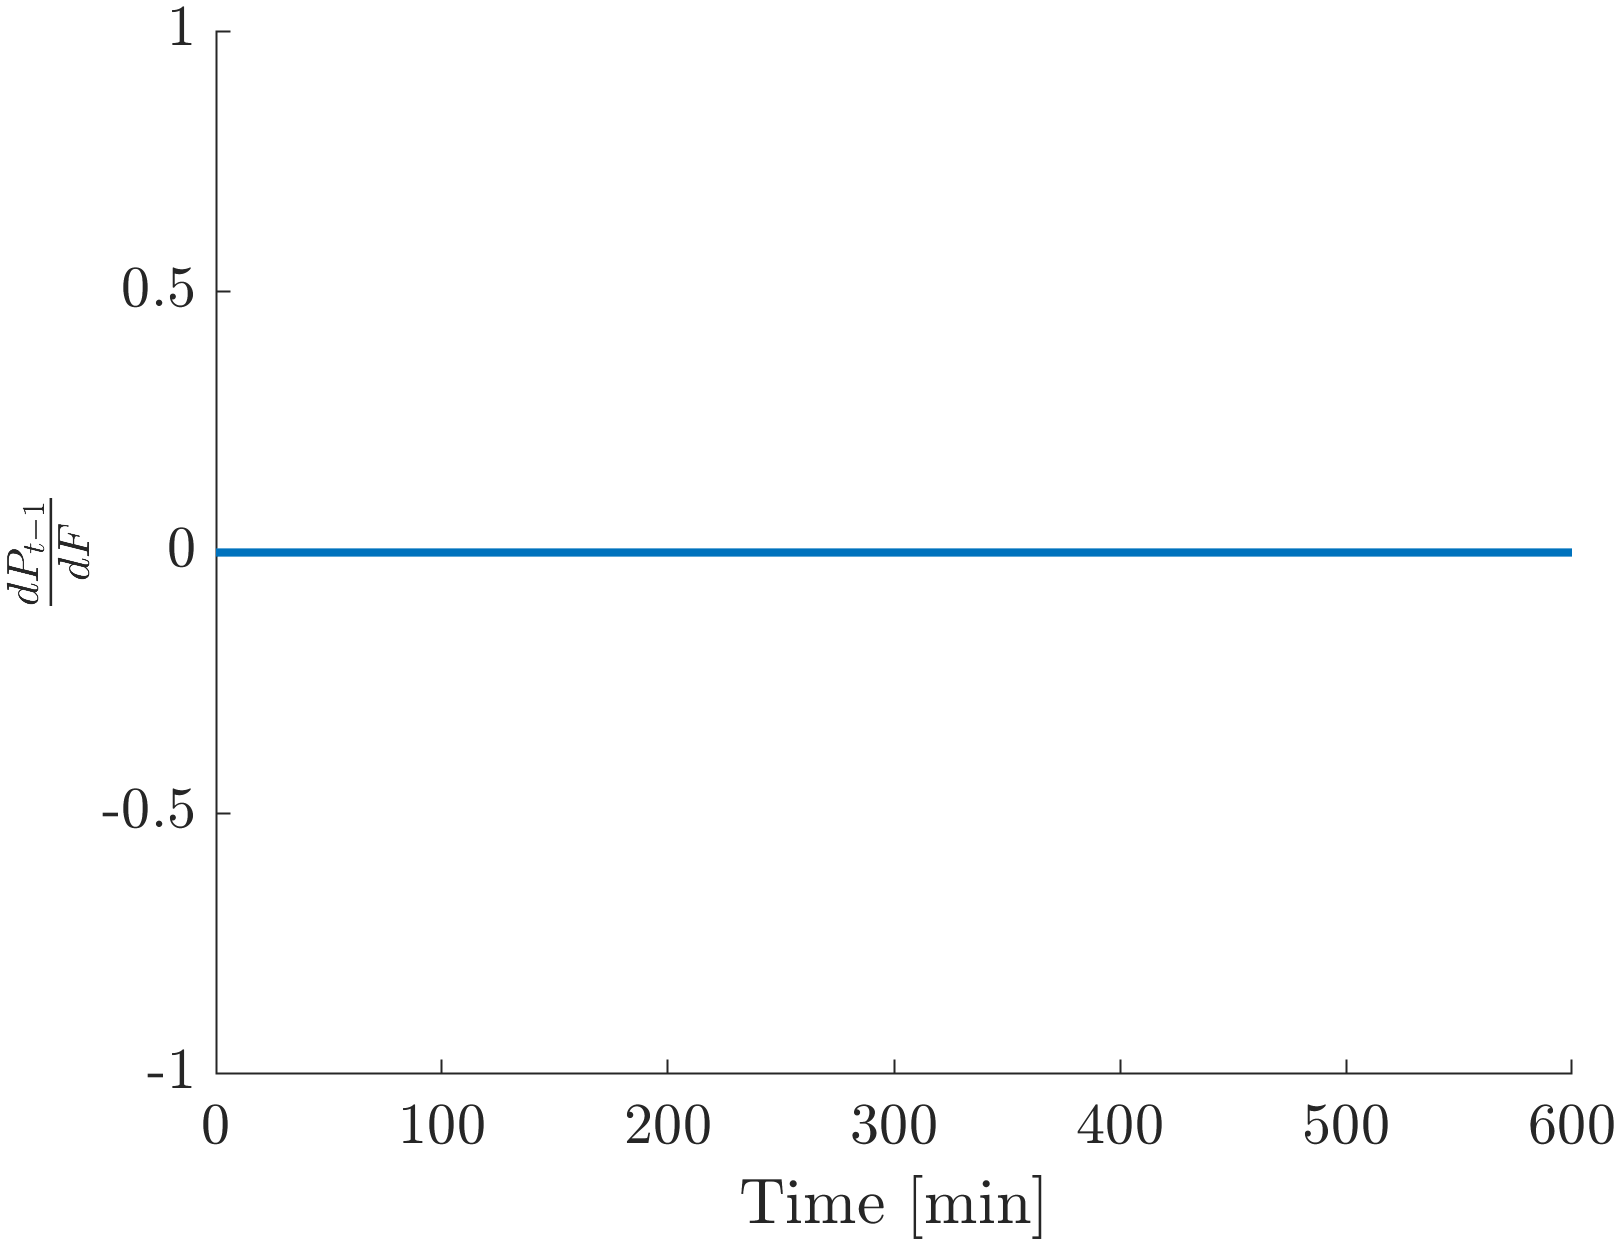
\includegraphics[trim = 0.0cm 0.0cm 0.0cm 0.0cm,clip,width=\columnwidth]{/Results_sensitivity/P_F.png}
		\caption{The effect of $F$ change on $P$}
		\label{fig:Sensitivty_F_P}
	\end{figure}
	
	It is important to note that $h$ represents enthalpy but not total enthalpy, thus excluding kinetic energy. As a consequence of the modelling assumptions, changes in $h$ and $\rho$ occur in response to changes in pressure or temperature, which explains no deviation of $h \times \rho$ in Figure \ref{fig:Sensitivty_F_H}.
	
	%When utilizing Dirichlet boundary conditions, it's crucial to be aware of potential numerical artefacts from the differing methods used to compute them. The system's enthalpy is determined through the time evolution of governing equations, while the inlet's enthalpy depends on the inlet temperature and pressure, which are the controls. A minor numerical mismatch between these values may manifest as an enthalpy difference propagating along the spatial domain. To ensure consistency between the fluid at the inlet and inside the computational domain, this analysis employs Neumann boundary conditions.
	
	\begin{figure}[h!]
		\centering
		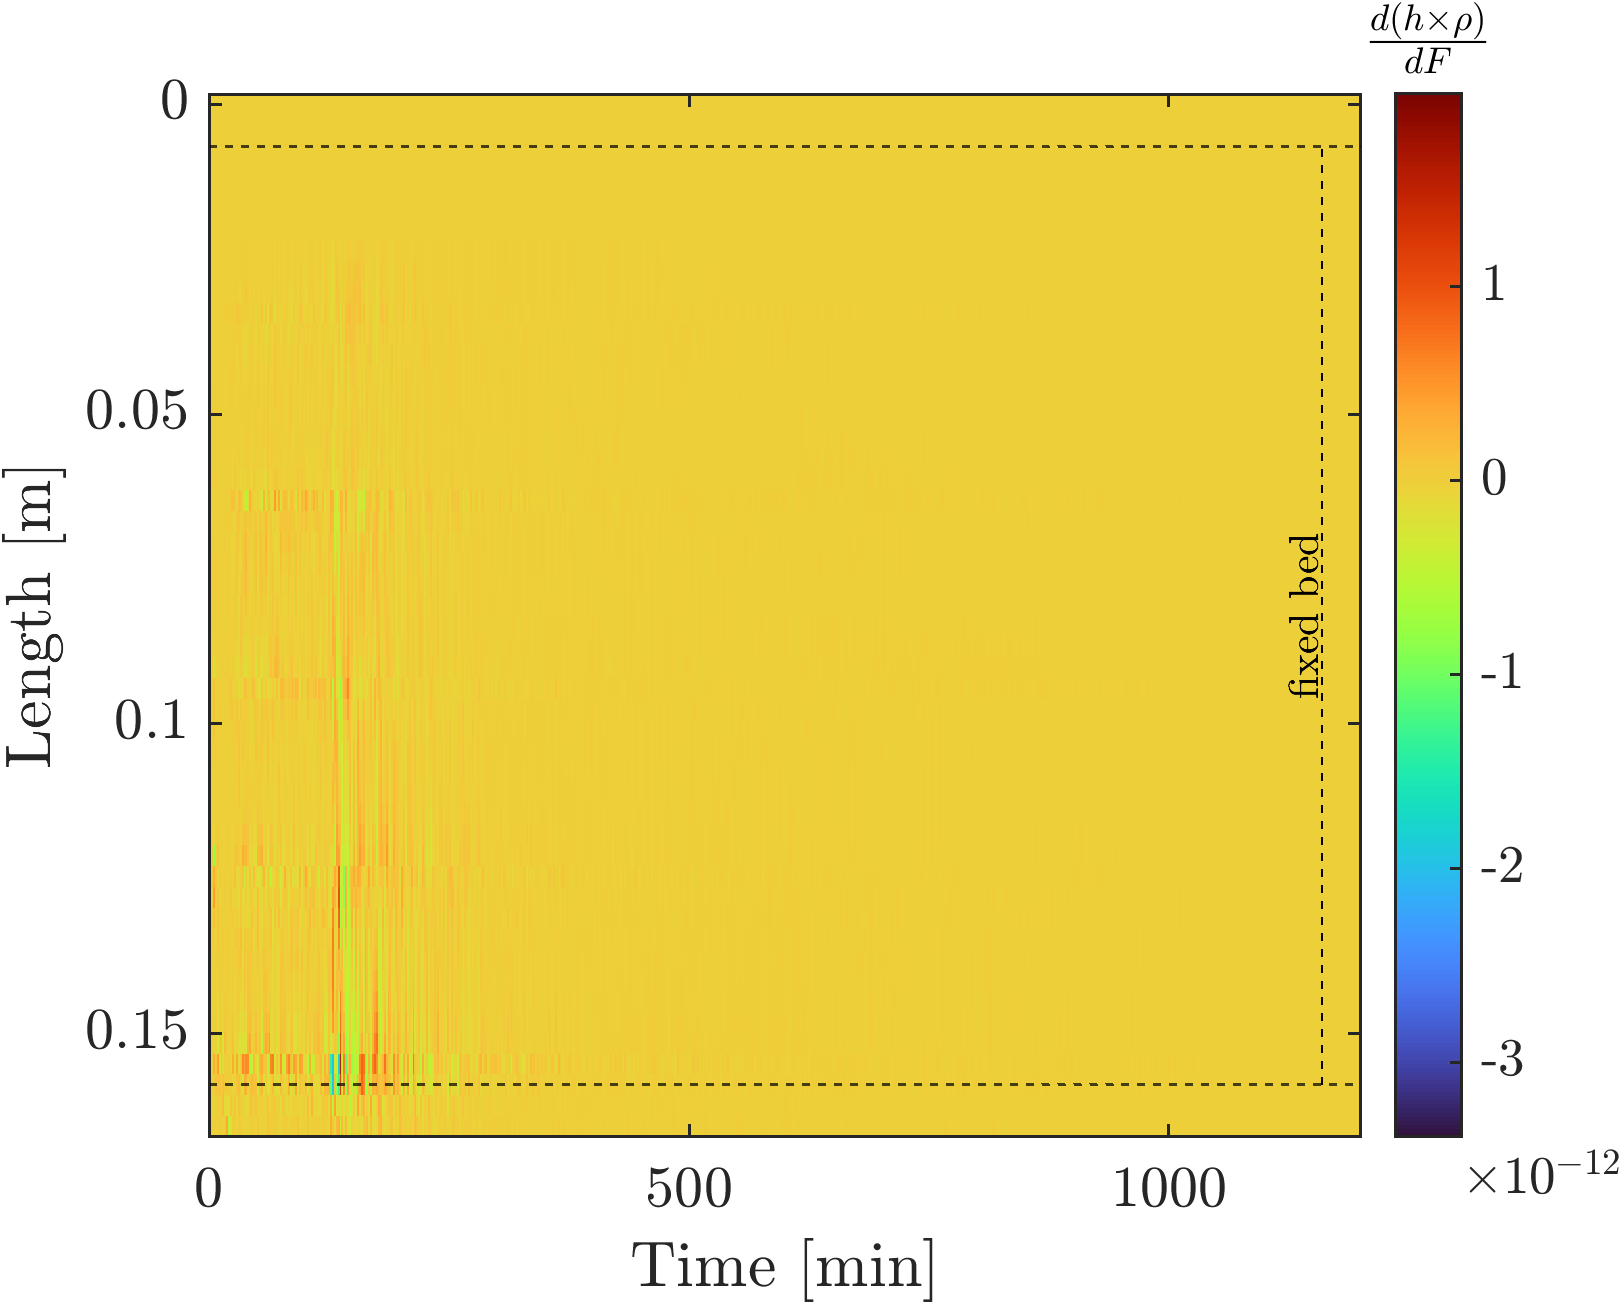
\includegraphics[trim = 0.0cm 0.0cm 0.0cm 0.0cm,clip,width=\columnwidth]{/Results_sensitivity/H_F.png}
		\caption{The effect of $F$ change on $h \times \rho$}
		\label{fig:Sensitivty_F_H}
	\end{figure}
	
	Figure \ref{fig:Sensitivty_F_CS} visualizes how the solute concentration in the solid phase is affected by the mass flow change. It is postulated that with an increase in the mass flow rate, the concentration gradient becomes larger leading to an accelerated decrease of the solute from solid particles and it is characterized by negative sensitivity values. Gradually, the sensitivities decrease until they reach minimum values and the effect of mass flow rate on extraction is most significant.
	
	\begin{figure}[h!]
		\centering
		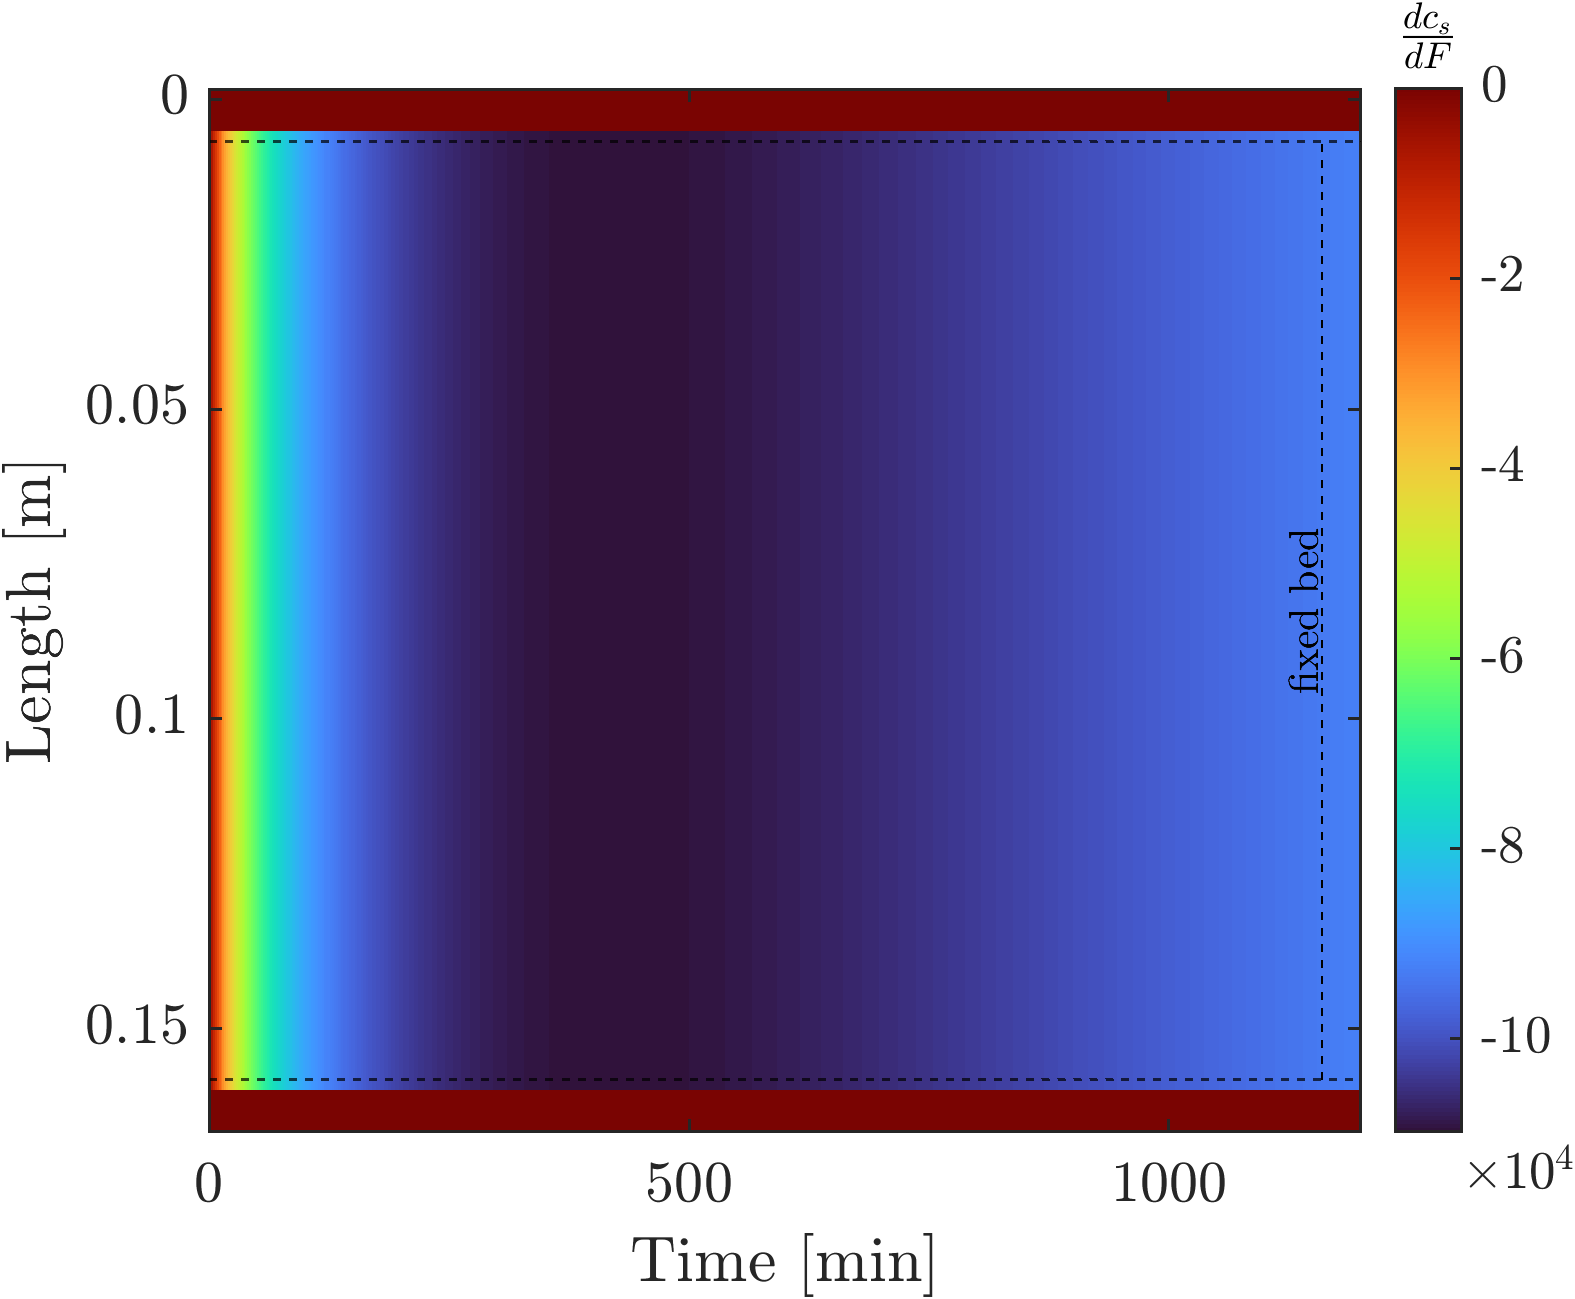
\includegraphics[trim = 0.0cm 0.0cm 0.0cm 0.0cm,clip,width=\columnwidth]{/Results_sensitivity/CS_F.png}
		\caption{The effect of $F$ change on $C_s$}
		\label{fig:Sensitivty_F_CS}
	\end{figure}
	
	As the extraction progresses, the sensitivity values become less negative, moving towards zero. This gradual change corresponds to the decreasing concentration of the solute in the solid phase, which results in a diminishing concentration gradient and, consequently, a reduction in the rate of extraction. The sensitivity approaching zero suggests that the driving force for mass transfer is decreasing as the solute is being depleted. The asymptotic behaviour can be interpreted as a point where the remaining solute concentration in the solid phase is minimal and becomes less dependent on the mass flow rate. At this stage, other factors, such as internal diffusion within the solid matrix or equilibrium limitations, may limit the extraction rate.
	
	%The asymptotic approach to zero sensitivity indicates a physical plateau in the extraction process, where further increases in mass flow rate no longer enhance the extraction efficiency. In practical terms, this asymptotic behavior signifies the approach towards an extraction endpoint where the remaining solute concentration in the solid phase is minimal and becomes less dependent on the mass flow rate. At this stage, other factors, such as diffusion within the solid matrix or equilibrium limitations, may limit the extraction rate.
	
	%In the most extreme cases, depicted by the uniform regions in the plot, the solute has been effectively exhausted, and the remaining traces in the solid phase are no longer influenced by changes in the mass flow rate. This stage represents the final equilibrium, where the concentration gradient effectively drops to zero, rendering the mass flow rate inconsequential for the extraction of the remaining solute. At this juncture, the system has reached its thermodynamic limit, and the efficiency of extraction cannot be enhanced by merely increasing the flow rate. This underscores the importance of optimizing the mass flow rate at the beginning and throughout the extraction process to ensure efficient solute recovery before reaching this terminal stage.
	
	%Figure \ref{fig:Sensitivty_F_CS} shows how the flow rate affects the solute concentration in the solid phase. At the beginning of the extraction process, the flow rate has a low impact on the extraction process due to the dominance of the concentration gradient in the kinetic regime. The corresponding sensitivities are close to zero. As time progresses, the increment in the mass flow rate has a greater influence on the extraction kinetics, causing the sensitivities to decrease towards their minimum values. Negative sensitivities indicate a faster extraction rate. 
	
	The Figure \ref{fig:Sensitivty_F_CF} depicts the sensitivity of the solute concentration in the fluid phase to the flow rate within a supercritical fluid extraction system. In the initial phase of the extraction, the sensitivities near the inlet are negligible, as characterized by values close to zero. This indicates a minimal initial response to changes in the flow rate, which could be due to the presence of an high concentration gradient, allowing the fluid phase to rapidly reach solute regardless of the flow rate.
	
	\begin{figure}[h!]
		\centering
		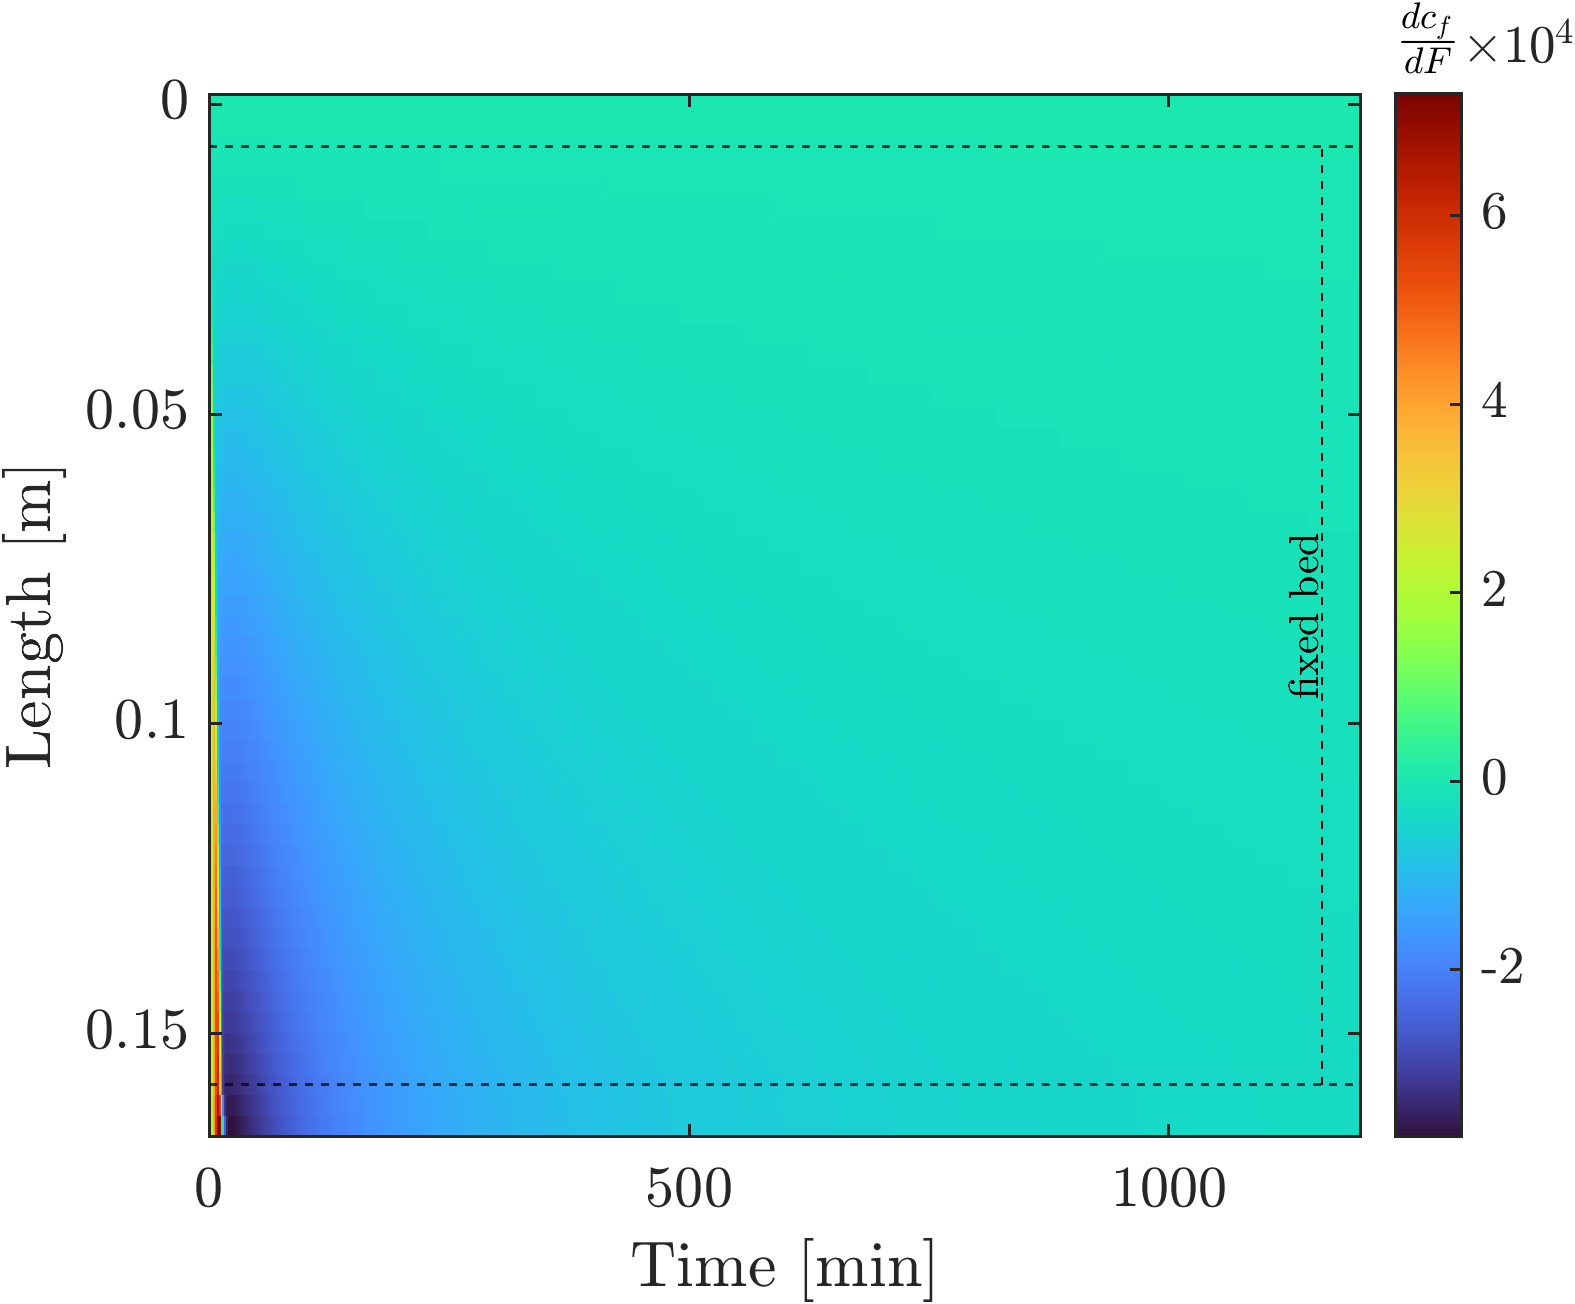
\includegraphics[trim = 0.0cm 0.0cm 0.0cm 0.0cm,clip,width=\columnwidth]{/Results_sensitivity/CF_F.png}
		\caption{The effect of $F$ change on $C_f$}
		\label{fig:Sensitivty_F_CF}
	\end{figure}
	
	As the extraction progresses, positive sensitivities emerge along the length of the extractor and form the concentration front that moves in the flow direction. This front represents the increased movement of the solute with the fluid phase as the flow rate increases, suggesting an enhanced mass transfer due to the elevated velocity of the supercritical fluid. Following the positive front, there is an emergence of a front characterized by negative sensitivities. This trend illustrates a diminishing solute concentration in the fluid phase, and it reflects a point in the extraction where the solute availability in the solid phase becomes a limiting factor; the depletion of solute reduces the concentration gradient, thereby decelerating the extraction rate. \todo{here}
	
	Toward the end of the extraction process, the sensitivities are shown to increase from their negative values towards zero. This asymptotic approach suggests that the system is reaching a kinetic regime where further increases in the flow rate have a low impact on the solute concentration in the fluid phase. This behavior reflects a physical limit where the remaining solute in the solid phase is insufficient to sustain a high concentration in the fluid phase, regardless of the flow rate. It indicates a terminal phase of the extraction process where the available solute has been largely exhausted, and the system response to changes in flow rate is inherently constrained by the depletion of extractable material.
	
	%Figure \ref{fig:Sensitivty_F_CF} shows how the concentration of solute in the fluid phase responds to an increase in the flow rate. Initially, sensitivities are close to zero, indicating a minimal system response. The growth in flow rate affects $C_f(z,t)$ indirectly by increasing the velocity and consequently elevating the concentration gradient. As a result, positive sensitivities emerge within the system, forming a front that progresses in the direction of flow. The positive front indicates that the larger amount of solute moves faster across the system. When the amount of the solute in the solid phase becomes a limiting factor, then the concentration gradient diminishes and slows down the extraction kinetics. The corresponding sensitivities form a front composed of negative sensitivities propagating through the extractor. The negative front indicates that the solute concentration in the fluid phase becomes lower than before the flow rate increment. Eventually, the negative sensitivities start to increase and asymptotically approach zero.
	
	The Figure \ref{fig:Sensitivty_F_y} depicts the sensitivity of the extraction yield to variations in mass flow rate  as a function of time. The curve’s initial rise to a peak followed by a decline conveys the dynamic relationship between the mass flow rate and the extraction yield within the supercritical extraction process.
	
	\begin{figure}[h!]
		\centering
		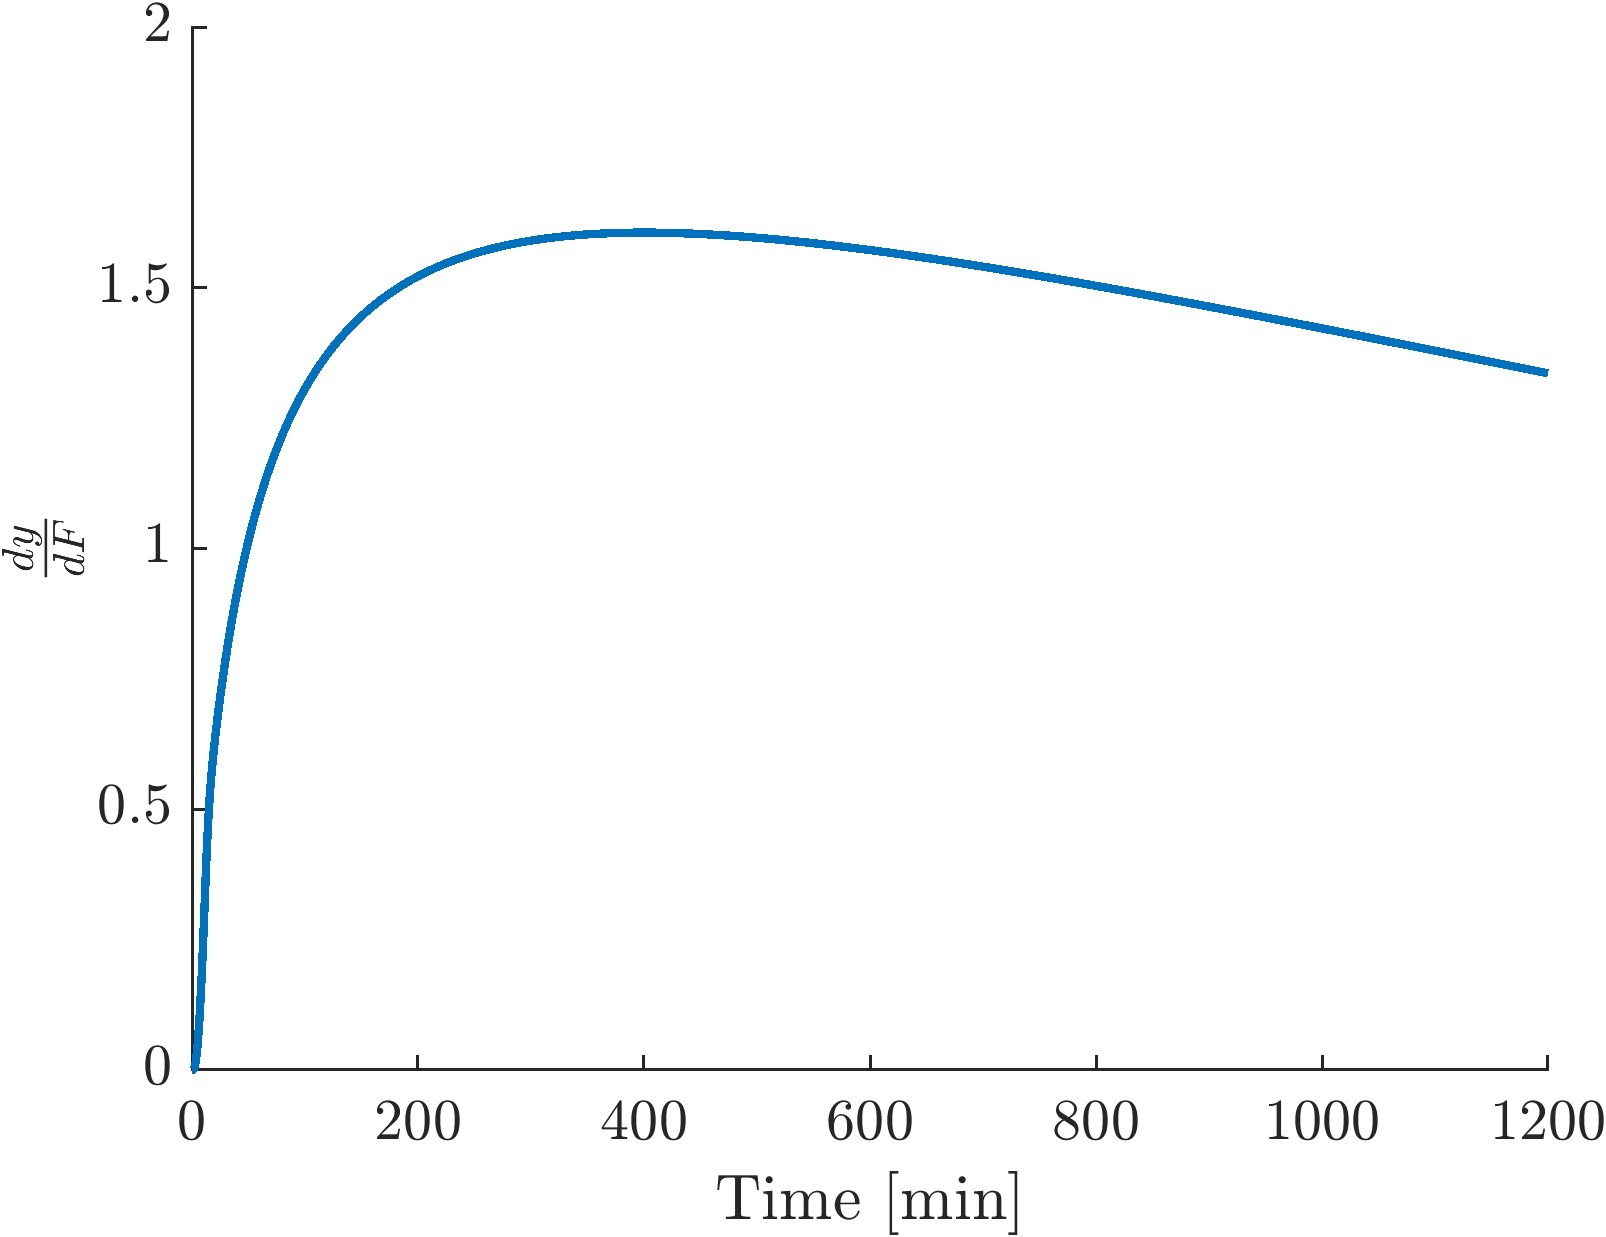
\includegraphics[trim = 0.0cm 0.0cm 0.0cm 0.0cm,clip,width=\columnwidth]{/Results_sensitivity/Y_F.png}
		\caption{The effect of $F$ change on $y(t)$}
		\label{fig:Sensitivty_F_y}
	\end{figure}
	
	In the early phase, the sensitivity is minimal, denoting that adjustments to the mass flow rate have a negligible influence on the yield. This can be attributed to the initial phase of the extraction, where the mass transport mechanisms are mainly controlled by a high concentration gradient.
	
	As the process evolves, the curve's ascent to its apex signifies a period during which the extraction yield becomes increasingly sensitive to the mass flow rate. This is likely due to the mass flow rate enhancing the convective transport of solute, maximizing the extraction efficiency. At this stage, the solute transfer from the solid to the fluid phase is most responsive to changes in flow rate.
	
	However, the curve’s descent past the peak suggests a diminishing return on sensitivity with further increases in mass flow rate. The decrease indicates a transitional phase where the extraction process likely encounters diffusion limitations or a depletion of readily extractable solute. The concentration gradient, which drives the mass transfer, may be reduced due to the depletion of solute in the solid phase, or the system may be experiencing diffusive resistances that limit the rate at which solute can be delivered to the fluid phase.
	
	The asymptotic approach to zero sensitivity towards the end of the curve reflects a regime where the yield is no longer significantly influenced by the mass flow rate. At this juncture, the extraction process has likely exhausted the available solute, and any further increase in mass flow rate does not result in a proportional increase in yield. The extraction system has reached a point of saturation or equilibrium where the mass transfer is limited by factors other than flow rate, such as the intrinsic properties of the solute or the matrix, indicating that the system has achieved as much extraction as is practically feasible under the given conditions.
	
	The curve captures the non-linear and transient nature of the extraction yield's response to the mass flow rate, underscoring the importance of optimizing flow rates over the duration of the extraction to maximize yield. It also highlights the multifaceted dependencies and constraints inherent in supercritical fluid extraction processes, such as mass transfer rates, solute availability, and diffusion limitations.
	
	%In Figure \ref{fig:Sensitivty_F_y}, the curve's shape reveals the time-dependent sensitivity of extraction yield to mass flow rate variations. The curve peaks and then falls, indicating a transient behavior in extraction efficiency. Initially, there's a negligible response, suggesting that changes in mass flow rate have little to no immediate impact on yield. As time progresses, however, yield becomes increasingly sensitive to the flow rate, reaching a peak sensitivity. Beyond this peak, the sensitivity decreases, which might reflect a saturation point in the extraction process where further increases in mass flow rate do not translate to increased yield, possibly due to limitations in solute diffusion rates from the solid matrix and decreasing concentration gradient. Eventually, $dy/dF$ asymptotically approaches zero. This happens because the amount of solute in the fluid phase becomes a limiting factor, and the process is in the diffusion regime.
	
\end{document}

